% DiagRAG: IEEE conference paper (IEEEtran, conference mode). Compile with: tectonic diagrag_ieee.tex
% Every number comes from a file in the repository (kaggle/judged_*/, kaggle/heldout_*/, docs/evidence/). Author names, affiliations,
% venue and the AI-assistance wording are the owner's decisions and are marked [OWNER].
\documentclass[conference]{IEEEtran}
\IEEEoverridecommandlockouts
\usepackage{cite}
\usepackage{amsmath,amssymb,amsfonts}
\usepackage{booktabs}
\usepackage{multirow}
\usepackage{graphicx}
\usepackage{url}
\usepackage{xcolor}
\usepackage{tikz}
\usepackage{pgfplots}
\pgfplotsset{compat=1.16}
\usetikzlibrary{arrows.meta,positioning,fit,calc}
\newcommand{\ci}[2]{[#1,\,#2]}
\newcommand{\tc}[1]{\texttt{#1}}
\newcommand{\PEND}[1]{\textcolor{red}{#1}}
\setlength{\tabcolsep}{3pt}

\begin{document}

\title{DiagRAG: Diagnosing and Repairing Retrieval Faults in RAG by Observation and Intervention, with Calibrated Risk Control and Empirical Harm Assessment}

\author{\IEEEauthorblockN{[OWNER: author name(s)]}
\IEEEauthorblockA{{[OWNER: affiliation]}\\
{[OWNER: e-mail]}}}

\maketitle

\begin{abstract}
When a retrieval-augmented generation (RAG) system answers badly, the cause often lies in retrieval, and retrieval rarely reports it. We study the detection, diagnosis and repair of retrieval faults using calibrated risk control and empirical harm assessment. For the per-query conformal gate, a per-stratum risk bound applies only to strata with at least 199 calibration examples; sparse strata use a pooled threshold and have no per-stratum guarantee. Held-out losses are empirical. Across nine GPU seeds, observed clean loss is at most 0.40\% for the stratified gate and 0.12\% for the capped variant; on the second stack, observed losses were 0.00\% for the original gate. We then ask what can be identified from what is observed. The telemetry of one query is one observation of the system, and the per-query diagnoser never names both causes of two faults in one group (0 of 75). A self-test using a known-answer probe battery names both causes in 85.3\% of 238 held-out same-group pairs and restores 99.7\% of traffic those pairs break, with 0.02\% observed harm. Passive decoding names both causes in 22.7\% on the same unique probes; this is not an equal-execution-budget comparison. Active runs used a median 672 probe executions (range 282--2{,}369), versus 102--103 unique probes in the battery; passive decoding with the same total number of executions was not evaluated. The second-stack pair result is 87\%, with all observed broken traffic restored and no observed harm. No acceptance-sampling certificate is claimed: repair selection and acceptance reused the probe outcomes. Among 301 repairs with measured traffic, 299 had observed harm below the nominal 2.95\% fixed-candidate value and two exceeded it, each breaking 1 of 23 queries. A diagnosability analysis explains the gap: passive decoding names both causes in 22.7\% on the same unique probes (not a matched execution budget), its success is predicted by a separability score computed from the fault dictionary alone (AUROC 0.74), and in the least separable third of pairs passive decoding names both causes in 4.4\%, compared with 86.7\% for the self-test. On nine retrieval bugs reproduced from public issue reports, the self-test detects 20 of 21 harmful bug-seed units, localizes all 21 and its verified rollback restores 1{,}454 of the 1{,}461 natural queries they break, while per-query telemetry alarms on 8. On code mutants of two retrieval code bases, the self-test detects all 32 harmful mutant runs (21 distinct mutants) and its stage trace localizes all scored ones, against 47\% for the fault dictionary. Telemetry alone detects injected faults at AUROC 0.977, against 0.734 for an existing system's retrieval features. Versioned protocols and code hashes document the experiments; subsequent amendments and exploratory analyses are identified separately, and negative outcomes are retained.
\end{abstract}

\begin{IEEEkeywords}
retrieval-augmented generation, fault diagnosis, conformal risk control, group testing, diagnosability, mutation testing, pre-registration
\end{IEEEkeywords}

%--------------------------------------------------------------------------------------------------
\section{Introduction}
RAG systems answer from documents they retrieve. When an answer is wrong the failure is often upstream: a misspelled query, near-duplicate passages that crowd out evidence, a stale vector index, a reranker that returns noise~\cite{barnett2024seven}. Retrieval logs scores but does not say that something is wrong, and evaluation frameworks that judge generated answers with a language model~\cite{es2023ragas,saadfalcon2024ares} need model calls per query and say little about where the fault is.

We study a narrow, testable problem: given what retrieval already exposes, (i) is retrieval faulty, (ii) which fault is it, (iii) which repair should run, and (iv) what harm does that repair cause on working queries? We measure held-out harm empirically and apply conformal risk control only within adequately calibrated per-query strata. A repair that fixes faulty queries but silently breaks working ones is worse than no repair; whether its harm can be bounded depends on the sampling and selection protocol.

The second question we ask is what can be identified at all. A diagnoser that sees one query sees one observation of the system. We show empirically that this is not enough to separate two faults of one kind, and that a small battery of probe queries with known answers, used actively (repair, then retest), is. The connection to group testing~\cite{dorfman1943,du2000group}, to diagnosability of discrete-event systems~\cite{sampath1995diagnosability} and to observation points in hardware test~\cite{bushnell2000essentials} gives a model that predicts which faults can be named from passive observation and why intervention helps.

\textbf{Contributions.}
\begin{enumerate}
\item \emph{Calibrated risk control with a qualified scope.} A per-stratum conformal risk-control gate for strata with sufficient calibration data; sparse strata use a pooled fallback without a per-stratum guarantee. Held-out loss and self-test repair harm are reported empirically (Sections~\ref{sec:gate} and~\ref{sec:res-gate}).
\item \emph{Observation versus intervention.} A measured limit of per-query diagnosis on composed faults, a diagnostic self-test that names both causes of same-group pairs and checks candidate repairs against a finite known-answer probe battery, and a diagnosability analysis that predicts passive identifiability from the fault dictionary alone (Sections~\ref{sec:selftest}, \ref{sec:res-composed}--\ref{sec:res-ladder}).
\item \emph{A telemetry diagnoser} for 32 injectable faults with detection and identification results against retrieval-stage, query-performance and LLM-judge baselines (Section~\ref{sec:res-diag}).
\item \emph{Evidence beyond designed faults}: nine retrieval bugs reproduced from public issue reports (95\% of harmful ones detected, all localized, accepted repairs pass the finite probe-battery check), code mutants of two retrieval code bases, real failures labelled by which repair fixes them, and never-examined natural traffic (Sections~\ref{sec:res-mutants} and~\ref{sec:res-real}).
\item \emph{Pre-registration throughout}: the code hash of every judged run, dated amendments, and every outcome, including the ones that failed (Section~\ref{sec:protocol}).
\end{enumerate}

%--------------------------------------------------------------------------------------------------
\section{Related Work}
\textbf{Diagnosis and repair of RAG.} RAGChecker diagnoses retriever versus generator with modular metrics~\cite{ru2024ragchecker}. Leung et al.\ give a taxonomy of RAG error types and an aligned auto-evaluation~\cite{leung2026ragec}. RAGLog localizes faults across RAG stages from execution logs with rule, embedding and LLM checks~\cite{raglog}; we use its retrieval-stage feature extractor as a baseline. D2R-RAG selects a corrective action under latency and memory budgets~\cite{hashemifar2026d2r}. AgenticRAG-FP injects a fault at a known hop of an agentic pipeline and scores diagnosers against it~\cite{pothuru2026agenticfp}. Corrective RAG grades documents with a model and rewrites the query~\cite{yan2024crag}. Metamorphic testing of RAG mutates the corpus to test consistency~\cite{kim2026metamorphic}. These systems use generated text or model calls, name a stage or an error type, and do not bound the harm of repair on healthy queries.

\textbf{Risk control.} Conformal risk control bounds the expected value of a monotone loss~\cite{angelopoulos2024crc}; Mondrian calibration gives the bound within strata~\cite{vovk2013mondrian}. C-RAG certifies generation risk of a RAG configuration~\cite{kang2024crag} and ToolChain-CRC calibrates an accept-or-intervene rule for agent trajectories~\cite{opoku2026toolchain}. From the abstracts we read, neither bounds the loss a repair causes on healthy queries.

\textbf{Diagnosis theory and testing.} Model-based diagnosis names minimal fault sets consistent with observations and uses probes to separate candidates~\cite{reiter1987theory,dekleer1987diagnosing}; diagnosability asks whether observations can separate faults at all~\cite{sampath1995diagnosability}. Group testing identifies defective items from pooled tests~\cite{dorfman1943,du2000group}, and noisy-OR networks model diagnosis with several causes~\cite{shwe1991qmr}. Hardware test generation chooses test patterns that distinguish faults and adds observation points to raise diagnosability~\cite{bushnell2000essentials}. Mutation testing judges test suites by the seeded faults they detect; mutants are a valid substitute for real faults in that use~\cite{just2014mutants,jia2011survey}, and higher-order mutants model interacting faults~\cite{jia2009hom}. The distinction between observing and intervening is central to causal identifiability~\cite{pearl2009causality}. We evaluate retrieval-only telemetry and active known-answer probes on injected, reproduced and mutated retrieval faults; the results do not establish a general repair-harm guarantee.

\textbf{Query performance prediction.} NQC~\cite{shtok2012qpp} and WIG~\cite{zhou2007wig} estimate retrieval quality without labels; we use both as baselines.

%--------------------------------------------------------------------------------------------------
\section{Setting}\label{sec:setting}
\textbf{Main stack.} Dense retrieval (bge-base-en-v1.5~\cite{xiao2023bge}) and BM25~\cite{robertson2009bm25} fused by reciprocal-rank fusion~\cite{cormack2009rrf} ($k{=}60$); the top 25 go to a cross-encoder reranker (bge-reranker-large), and five are returned. A query \emph{succeeds} if a gold document is in the top five (Hit@5). The corpus has 101{,}297 documents; the queries are Amazon ESCI shopping queries~\cite{reddy2022esci} (about 88\% of episode bases; the rest are product-catalogue, FAQ and documentation texts of the same corpus, not released). \textbf{Second stack.} e5-small-v2 in an HNSW index, BM25, min-max fusion and a MiniLM reranker, on BEIR FiQA and NQ~\cite{thakur2021beir} (2.68M passages).

\textbf{Fault model.} 32 injectable faults in four groups: query (Q), knowledge base (K), retrieval stack (R) and composition (C); the adoption rule counts the \emph{core 28} (Table~\ref{tab:faults}). Each fault is tied to public field reports by an evidence tier. Real misspellings come from Webis-QSpell-17~\cite{hagen2017qspell}. An \emph{episode} runs a query through the clean and the faulted pipeline and is kept only if the clean one succeeds and the faulted one fails; splits are by gold-product component.

\begin{table}[t]
\caption{Core faults by group.}
\label{tab:faults}
\centering\footnotesize
\begin{tabular}{@{}p{0.07\columnwidth}p{0.85\columnwidth}@{}}
\toprule
Group & Faults\\
\midrule
Q & Q01 unfinished last word; Q02 chatty filler; Q03 paraphrase by another real user; Q04 misspelling; Q05 missing space; Q07 corrupted model number; Q09 two needs in one query\\
K & K03 sibling products with one identity; K04 stale vector; K05 near-duplicates; K06 unverified copies; K07 other-tenant leak; K08 placeholder documents; K09 expired versions\\
R & R01 index coverage hole; R03 encoder truncation; R05 reranker returns garbage; R06 misrouting; R07 shifted embedding rows; R10 query-vector noise; R11 encoder drift; R13 BM25 dictionary out of sync; R15 ANN recall; R19 rerank depth cut; R22 raw-score fusion; R23 partial results; R24 reranker truncation\\
C & C2 two faults from different groups\\
\bottomrule
\end{tabular}
\end{table}

%--------------------------------------------------------------------------------------------------
\section{Method}\label{sec:method}
\subsection{Per-query telemetry diagnoser}
Each query yields 63 numbers from the retrieval trace only (no gold label, no generated answer): query features, score gaps of the dense, sparse and reranker legs, agreement between legs, duplicate and chunk-crowding counts, filter checks and cheap probes (approximate-versus-exact recall, vector alignment, a stale-vector probe). A histogram gradient-boosted attributor~\cite{pedregosa2011sklearn} scores the clean class and every fault. A dispatcher applies a fired precise rule first; otherwise it picks the fault group by probability mass, then the repair family inside the group, with a group repair as fallback. Each fault has a repair (spelling correction, segmentation, near-duplicate collapse, re-applying a filter, rebuilding the dense view, restoring fusion, and so on).

\subsection{Do-no-harm gate}\label{sec:gate}
Let $s$ be the attributor's fault score and $\ell(\lambda)\in\{0,1\}$ the Hit@5 lost on a healthy query when its repair is dispatched at threshold $\lambda$. Conformal risk control~\cite{angelopoulos2024crc} chooses the smallest threshold satisfying $\frac{n}{n+1}\hat{\mathbb{E}}[\ell(\lambda)]+\frac{1}{n+1}\le\alpha$, with $\alpha{=}0.005$, using calibration queries not used to fit the attributor. Under exchangeability, this targets expected loss at most $\alpha$ within a calibration stratum. The capped variant raises each threshold until at most 20\% of calibration queries are dispatched; this preserves the risk bound where that stratum has sufficient calibration data. At least $\lceil(1-\alpha)/\alpha\rceil{=}199$ examples are needed for a finite threshold at this $\alpha$. When a stratum has fewer than 199 examples, the pipeline uses the pooled threshold as a fallback. This fallback is not a stratum-specific conformal procedure and carries no per-stratum risk guarantee; its held-out loss is empirical.

\subsection{Diagnostic self-test}\label{sec:selftest}
Faults of the retrieval system itself (the encoder, the index, BM25, fusion, the reranker and serving settings) affect every query. For them we add an active test, built from the ideas of hardware test and laboratory quality control. Figure~\ref{fig:selftest} shows the loop.

\textbf{Probes.} The probes are training queries with known answers that the clean pipeline retrieves. A battery has 100 random probes plus a few chosen greedily so that the failure signatures of every pair of faults differ.

\textbf{Fault dictionary.} For each of 15 system faults we inject it, with its own random parameters, and record which probes fail; $q_{f,i}$ is the failure rate of probe $i$ under fault $f$. Under a noisy-OR model a set $H$ of faults makes probe $i$ fail with probability $p_i(H)=1-(1-\epsilon)\prod_{f\in H}(1-q_{f,i})$.

\textbf{Repair and retest.} The self-test runs the battery. If probes fail, it ranks faults by the likelihood of the observed failures, tries the repairs of the six most likely (then their pairs) on the failing probes, keeps the one that fixes most, and confirms it on the whole battery; it repeats up to four rounds, then rolls back to the pinned configuration. A repair is accepted only if every probe passes again.

\textbf{Repair-harm assessment.} For a repair fixed independently of a fresh sample, an untouched sample of $n$ exchangeable working queries with zero observed harms would yield the one-sided 95\% Clopper--Pearson upper bound $1-0.05^{1/n}$ (2.95\% at $n{=}100$). The implemented adaptive search selects and accepts repairs using outcomes on the same probe battery. It therefore does not meet the fixed-candidate, independent-sample condition, and we claim no 95\% system-repair certificate. We report observed harm on the measured traffic sample. The conformal claim applies only to adequately calibrated per-query strata, as qualified above.

\textbf{Stage-traced localization.} For a fault outside the dictionary, the self-test records the output of every stage for each probe (dense top-20, sparse top-20, fused list, reranked top-10, served top-5) and compares it with the clean run. The earliest stage whose output changes names the component (dense and sparse both changed: the filters). These are observation points in the sense of hardware test.

\begin{figure}[t]
\centering
\resizebox{\columnwidth}{!}{%
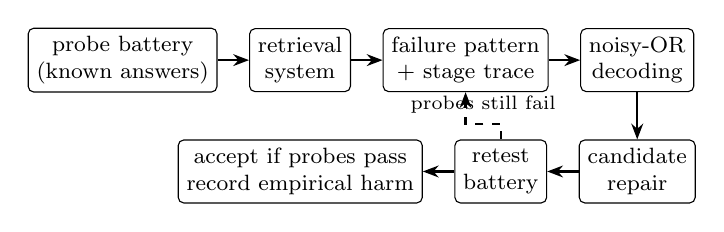
\begin{tikzpicture}[node distance=4mm, box/.style={draw, rounded corners=2pt, align=center, minimum height=8mm, font=\footnotesize, inner sep=3pt}, arr/.style={-{Stealth[length=2mm]}, thick}]
\node[box] (p) {probe battery\\(known answers)};
\node[box, right=of p] (r) {retrieval\\system};
\node[box, right=of r] (y) {failure pattern\\+ stage trace};
\node[box, right=of y] (d) {noisy-OR\\decoding};
\node[box, below=6mm of d] (rep) {candidate\\repair};
\node[box, left=of rep] (ret) {retest\\battery};
\node[box, left=of ret] (acc) {accept if probes pass\\record empirical harm};
\draw[arr] (p)--(r); \draw[arr] (r)--(y); \draw[arr] (y)--(d); \draw[arr] (d)--(rep); \draw[arr] (rep)--(ret); \draw[arr] (ret)--(acc);
\draw[arr, dashed] (ret.north) -- ++(0,2mm) -| node[pos=0.25, above, font=\scriptsize]{probes still fail} (y.south);
\end{tikzpicture}}
\caption{Diagnostic self-test. Probes with known answers are run, their failures decoded against a fault dictionary, a candidate repair is applied and the battery is re-run; a repair is accepted only when every probe passes, which validates only against this finite battery.}
\label{fig:selftest}
\end{figure}

%--------------------------------------------------------------------------------------------------
\section{Protocol}\label{sec:protocol}
Before each judged run a protocol file records the gates, the configuration and the SHA-256 of the exact code; amendments are dated and committed before the results they touch. A pipeline run is \emph{adopted} if at least 27 of 28 core detectors (held-out AUROC $\ge0.70$, $\ge50$ positives) and 24 of 28 repairs (Wilson lower bound of rescue $\ge0.50$, at most 10\% of clean successes lost) pass. Each new method was developed on seed 55 (later mutant development also on the seed-71 and seed-72 pipelines, using only the development half of the mutants) and confirmed on data it had not touched (seeds 71--73, then 74--76); its pass rule was written after development and before confirmation. Proportions use Wilson intervals~\cite{wilson1927} and differences paired bootstrap intervals. Baselines: RAGLog tier-0 features with the same classifier~\cite{raglog}; NQC, WIG and the top reranker score; three zero-shot LLM judges; a diagnosis-free universal repair applied to every query; SymSpell and word segmentation; a CRAG-style repair. All runs use free Kaggle GPUs; no paid model is used. The code, experiments and text were produced with an AI assistant (Section~\ref{sec:ethics}).

%--------------------------------------------------------------------------------------------------
\section{Results}\label{sec:results}
\subsection{Adoption across nine seeds}
Table~\ref{tab:runs} lists every judged pipeline run of the final configuration. Eight of nine GPU seeds are adopted; seed 52 misses on Q03 (AUROC 0.618) and C2 (0.681). A pre-registered seed-averaged rule (mean AUROC per detector over the three untouched seeds 71--73, pooled repair counts) also adopts: only Q03 fails (mean 0.638). Q03, a paraphrase typed by another real user, leaves almost no trace in telemetry and fails in every run.

\begin{table}[t]
\caption{Judged runs of the final configuration. Det./Rep. = core detectors and repairs passing (of 28). L1: held-out clean loss of the stratified gate (bar 0.5\%); Cap.: clean loss of the capped gate; L2: closure of injected faults; U1: closure of faults the attributor never saw (bar 0.50); N1: natural-traffic gain, Hit@5 points.}
\label{tab:runs}
\centering\footnotesize
\begin{tabular}{@{}llccccccl@{}}
\toprule
Seed & Stack & Det./Rep. & L1 & Cap. & L2 & U1 & N1 & Verdict\\
\midrule
50 & GPU & 27/27 & 0.28\% & 0.12\% & 0.844 & 0.406 & $+2.18$ & adopted\\
50 & CPU & 28/27 & 0.20\% & 0.08\% & 0.854 & 0.413 & $+2.43$ & adopted\\
52 & GPU & 26/27 & 0.40\% & 0.12\% & 0.886 & 0.397 & $+2.06$ & \textbf{not}\\
55 & GPU & 27/27 & 0.16\% & 0.08\% & 0.865 & 0.396 & $+2.00$ & adopted\\
71 & GPU & 27/26 & 0.16\% & 0.08\% & 0.856 & 0.398 & $+2.06$ & adopted\\
72 & GPU & 27/27 & 0.16\% & 0.12\% & 0.856 & 0.403 & $+2.12$ & adopted\\
73 & GPU & 27/27 & 0.12\% & 0.04\% & 0.859 & 0.408 & $+2.00$ & adopted\\
74 & GPU & 27/27 & 0.16\% & 0.08\% & 0.863 & 0.381 & $+2.00$ & adopted\\
75 & GPU & 27/27 & 0.12\% & 0.08\% & 0.854 & 0.378 & $+2.06$ & adopted\\
76 & GPU & 27/27 & 0.16\% & 0.04\% & 0.833 & 0.361 & $+2.00$ & adopted\\
\bottomrule
\end{tabular}
\end{table}

\subsection{Empirical harm and conformal risk control}\label{sec:res-gate}
Across evaluated held-out seeds, observed clean loss was at most 0.40\% for the stratified gate and 0.12\% for the capped gate (Table~\ref{tab:runs}); this is empirical, not proof that every fallback stratum meets the target. Table~\ref{tab:policy} and Fig.~\ref{fig:pareto} show the observed closure-cost trade-off on one seed. The stratified gate dispatches on 85\% of clean queries; the capped gate has 0.08\% observed clean loss at 16.1\% dispatch and closure 0.838, against 1.63\% loss, cost 12 and closure 0.761 for the universal repair. An un-stratified global threshold has 0.64\% observed clean loss in this run; this does not validate pooled fallback within a sparse stratum. The capped variant was designed after the stratified one.

\begin{table}[t]
\caption{Dispatch policies on held-out queries (CPU run, seed 50). Cost: repair cost per clean query (illustrative weights Q=1, K=3, R=8). Closure is over injected faults.}
\label{tab:policy}
\centering\footnotesize
\begin{tabular}{@{}lcccc@{}}
\toprule
Policy & Clean loss & Dispatch & Cost & Closure\\
\midrule
5\% false-positive threshold (no bound) & 0.16\% & 3.3\% & 0.17 & 0.847\\
global CRC, $\alpha{=}0.005$ & 0.64\% & 44.4\% & 2.36 & 0.892\\
stratified CRC, $\alpha{=}0.0025$ & 0.16\% & 66.6\% & 3.08 & 0.587\\
stratified CRC, $\alpha{=}0.005$ & 0.16\% & 85.4\% & 4.03 & 0.846\\
stratified CRC, $\alpha{=}0.02$ & 0.40\% & 89.0\% & 4.22 & 0.887\\
\textbf{capped CRC, $\alpha{=}0.005$} & \textbf{0.08\%} & \textbf{16.1\%} & \textbf{1.03} & \textbf{0.838}\\
universal repair, every query & 1.63\% & 100\% & 12.00 & 0.761\\
\bottomrule
\end{tabular}
\end{table}

\begin{figure}[t]
\centering
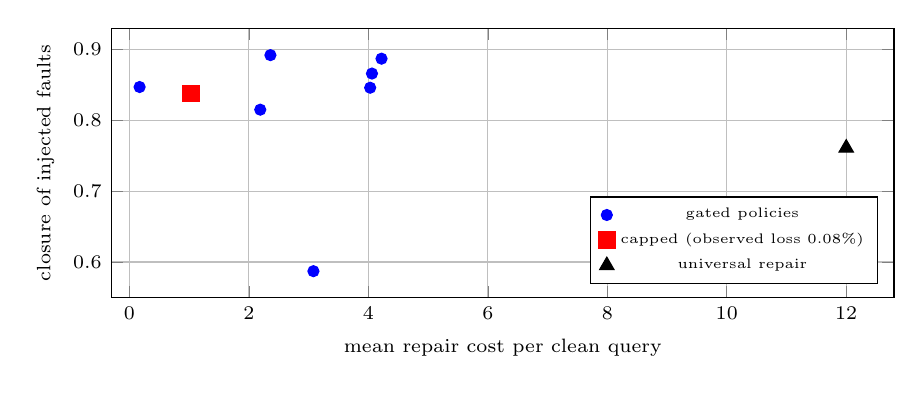
\begin{tikzpicture}
\begin{axis}[width=0.95\columnwidth,height=5.0cm,xlabel={mean repair cost per clean query},ylabel={closure of injected faults},xmin=-0.3,xmax=12.8,ymin=0.55,ymax=0.93,grid=major,tick label style={font=\scriptsize},label style={font=\scriptsize},legend style={font=\tiny,at={(0.98,0.05)},anchor=south east}]
\addplot[only marks,mark=*,blue] coordinates {(0.17,0.847)(2.36,0.892)(3.08,0.587)(4.03,0.846)(4.06,0.866)(4.22,0.887)(2.19,0.815)};
\addlegendentry{gated policies}
\addplot[only marks,mark=square*,red,mark size=3pt] coordinates {(1.03,0.838)};
\addlegendentry{capped (observed loss 0.08\%)}
\addplot[only marks,mark=triangle*,black,mark size=3pt] coordinates {(12.0,0.761)};
\addlegendentry{universal repair}
\end{axis}
\end{tikzpicture}
\caption{Closure against cost for the dispatch policies (CPU run, seed 50). The capped gate reaches 0.838 closure at cost 1.03 with 0.08\% observed clean loss; the universal repair reaches 0.761 at cost 12 with 1.63\% observed clean loss.}
\label{fig:pareto}
\end{figure}

\textbf{Second stack.} We re-calibrated the gate on the second stack (FiQA, NQ; 20 of the 32 faults ported; a pre-registered replay of the judged port runs). Table~\ref{tab:stack2} gives the result. Observed held-out clean loss was 0.00\% for the gated policies on both corpora (Wilson upper bound 0.31\%); this is empirical and does not establish a per-stratum guarantee for sparse strata. The capped gate on FiQA missed the pre-registered closure bar (0.690 against 0.70), because the rare-vocabulary stratum had 71 calibration queries on FiQA and 16 on NQ, both below the 199-example threshold requirement. One of two strata per corpus therefore used a pooled fallback, with no per-stratum guarantee. The observed capped-fallback loss/closure was 0.08\%/0.892 on FiQA and 0.00\%/0.909 on NQ. The universal repair breaks 2.2 to 2.4\% of healthy queries and is about 70 times slower than a dispatched repair on FiQA (0.63\,s against 0.009\,s per query).

\begin{table}[t]
\caption{Per-query dispatch gate on the second stack, held-out test queries (FiQA $n{=}1257$, NQ $n{=}1250$ clean). Closure over the 20 ported faults.}
\label{tab:stack2}
\centering\footnotesize
\begin{tabular}{@{}llccc@{}}
\toprule
Corpus & Policy & Clean loss & Dispatch & Closure\\
\midrule
FiQA & stratified CRC & 0.00\% & 96.3\% & 0.700\\
     & capped CRC & 0.00\% & 21.1\% & \textbf{0.690} (bar 0.70)\\
     & capped + pooled fallback$^{\dagger}$ & 0.08\% & 24.3\% & 0.892\\
     & universal repair & 2.23\% & 100\% & 0.888\\
NQ   & stratified CRC & 0.00\% & 99.2\% & 0.756\\
     & capped CRC & 0.00\% & 20.3\% & 0.742\\
     & capped + pooled fallback & 0.00\% & 21.1\% & 0.909\\
     & universal repair & 2.40\% & 100\% & 0.882\\
\bottomrule
\multicolumn{5}{@{}l}{\footnotesize $^{\dagger}$Pooled fallback applies to the rare stratum only (FiQA $n{=}71$ of 2,632 calibration examples; NQ $n{=}16$ of 1,568); displayed losses and closures are empirical, with no per-stratum guarantee there.}
\end{tabular}
\end{table}

\subsection{Detection and identification}\label{sec:res-diag}
On 4{,}019 held-out episodes (CPU run, seed 50) the attributor separates faulted from clean episodes at AUROC 0.977 $\ci{0.972}{0.981}$, against 0.734 for RAGLog's retrieval-stage features with the same classifier, 0.551 for its best single feature, 0.632 for the negated top reranker score and 0.55 to 0.57 for NQC and WIG. On 320 held-out episodes of an earlier run, zero-shot LLM judges that see the query and the five documents reach 0.754 (Gemini 3.1 Flash-Lite), 0.701 (gpt-oss-120b) and 0.629 (gpt-oss-20b), against 0.975 for the attributor on the same episodes; this is supervised against zero-shot, and no frontier model was run. As a 32-class identifier, the attributor names the exact fault in 89.9\% of faulted episodes (macro-F1 0.896); of its errors, 127 are faults called clean and only 26 are confusions between two faults. F1 is at least 0.90 for 22 of 31 faults; Q03 is never identified. Table~\ref{tab:perfault} gives every fault. On the second stack, top-1 identification of faulted episodes is 0.932 (FiQA) and 0.959 (NQ).

\begin{table}[t]
\caption{Per-fault F1 of the attributor, held-out (CPU run, seed 50; 50 episodes per fault except R26, 11). Clean class: F1 0.95.}
\label{tab:perfault}
\centering\footnotesize
\begin{tabular}{@{}lc@{\hspace{6pt}}lc@{\hspace{6pt}}lc@{\hspace{6pt}}lc@{}}
\toprule
Fault & F1 & Fault & F1 & Fault & F1 & Fault & F1\\
\midrule
Q01 & 0.82 & K03 & 0.99 & R01 & 1.00 & R15 & 0.98\\
Q02 & 0.97 & K04 & 0.78 & R03 & 0.95 & R19 & 0.99\\
Q03 & 0.00 & K05 & 0.95 & R05 & 0.96 & R22 & 0.80\\
Q04 & 0.72 & K06 & 1.00 & R06 & 0.85 & R23 & 1.00\\
Q05 & 0.69 & K07 & 1.00 & R07 & 0.90 & R24 & 0.73\\
Q07 & 0.89 & K08 & 0.97 & R10 & 0.99 & R25 & 1.00\\
Q09 & 0.96 & K09 & 1.00 & R11 & 0.96 & R26 & 0.95\\
    &      & K11 & 1.00 & R13 & 0.98 & K12 & 0.94\\
\bottomrule
\end{tabular}
\end{table}

\subsection{The limit of per-query diagnosis on composed faults}\label{sec:res-composed}
In a pre-registered study of 155 held-out composed episodes (pairs and triples of the 20 grounded faults, eight strata, seed 51), the retrained attributor names every cause in 40.0\% $\ci{32.6}{47.9}$ of episodes and at least one in 96.1\%. It names \textbf{0 of 75} pairs inside one fault group and triples: the dispatcher returns one label per group. Sequential repair (repair, re-diagnose, repair) still closes 72.9\% against 83.9\% when the true causes are repaired in order, because one group repair often fixes both causes. In 25.8\% of episodes neither fault breaks retrieval alone. Adding composed training rows caused no regression on the single-fault gates.

\subsection{The diagnostic self-test}\label{sec:res-selftest}
We evaluated the self-test on the 15 system faults (three random instances each) and on all 104 pairs that do not set the same configuration knob, on three untouched pipeline seeds (71--73). An instance is \emph{harmful} if it breaks at least one of 100 working test queries, a pair \emph{effective} if each fault alone is harmful; names are scored at the level of the repair family. The pass rule, five conditions, was fixed after development on seed 55. Table~\ref{tab:selftest} gives the held-out result: all five conditions hold.

\begin{table}[t]
\caption{Self-test, held-out (seeds 71--73 pooled). Harmful single faults $n{=}125$; effective pairs $n{=}270$ (238 in one fault group). Traffic: 100 test queries per instance (40 per pair). Loop = frozen per-query diagnoser with its gate.}
\label{tab:selftest}
\centering\footnotesize
\begin{tabular}{@{}lccc@{}}
\toprule
 & Self-test & Loop & Universal\\
\midrule
Single faults detected & 99.2\% & & \\
Right fault family named & 99.2\% & & \\
Finite probe battery passed (singles / pairs) & 100\% / 100\% & & \\
Both causes named, same-group pairs & \textbf{85.3\%} & 25.6\%$^{*}$ & --\\
Traffic closure, single faults & 97.0\% & 95.1\% & 96.2\%\\
Traffic closure, pairs & 99.7\% & 58.1\% & 98.9\%\\
Harm on working queries, singles & 0.00\% & 0.27\% & 4.23\%\\
Harm on working queries, pairs & 0.02\% & 6.27\% & 1.33\%\\
\bottomrule
\multicolumn{4}{@{}l}{\footnotesize $^{*}$Per-query labels aggregated over the traffic (two most frequent families).}
\end{tabular}
\end{table}

Same-group pairs are named in 88\%, 87\% and 80\% on the three seeds; the difference to the aggregated per-query labels is $+0.60$ $\ci{+0.53}{+0.67}$. Faults removed from the dictionary are named in 88.6\% of cases when a fault with the same repair family remains. Against the universal repair the self-test wins on harm (0.00 to 0.02\% against 1.3 to 4.2\%) more than on closure. One fault (R07, shifted vectors in a block of 20{,}000 documents) breaks almost no probe and is not detected on seed 72. A self-test takes a median of 4.8\,s and about 390 probe runs. Harm measurements are empirical. Across 301 repairs with measured traffic, 299 (99.3\%) had observed harm below the nominal 2.95\% fixed-candidate value; two exceeded it, each breaking 1 of 23 queries. Because repair selection and acceptance reused probe outcomes, the fixed-candidate Clopper--Pearson calculation does not certify these adaptive repairs. No untouched independent certification sample was used.

\textbf{Second stack.} The same algorithm, with the second stack's 14 system faults and repairs, was developed on FiQA and confirmed on FiQA with held-out fault draws (the planned NQ confirmation could not finish before the freeze, because an NQ retrieval is about 40 times slower; this fallback was fixed in advance). The rule was the same five empirical conditions, with two disclosed changes made before the held-out run: the per-query baseline of this stack has no gate, so the self-test must not fall below it on single faults rather than exceed it, and closure is the pooled share of broken traffic queries restored (on development the per-instance mean was dominated by one instance with one broken query; on the held-out run both measures are 1.000). All five conditions hold. Detection 27 of 27 harmful single faults, family named 96.3\%, every accepted repair passed the finite probe-battery check; both causes named in 87.0\% of 23 same-group pairs against 39.1\% for aggregated per-query labels ($+0.48$ $\ci{+0.22}{+0.74}$); the self-test restores all 117 and all 152 broken traffic queries of single faults and pairs, against 99.3\% and 49.7\% for the per-query baseline and 90.3\% and 59.7\% for the universal repair, with no harm (per-query baseline 0.5\% and 9.4\%, universal repair 4.4\% and 7.4\%). K04 is not detectable by this stack's battery.

\subsection{Why intervention identifies what observation cannot}\label{sec:res-ladder}
We replayed the same fault instances and probes and decoded them \emph{passively}: maximum-likelihood decoding of the failure pattern under the noisy-OR dictionary, with no repair, from $m$ random probes. For a pair $T$ we computed, from the dictionary alone, its separability $D(T)$: the smallest summed Kullback--Leibler divergence between the outcome distribution of $T$ and that of any explanation that does not cover both causes. Under the noisy-OR model the error of passive decoding falls as $D$ grows, and $D$ grows with the number of probes. Four predictions were fixed after development on seed 55 and before the held-out run; all four hold on seeds 71--73 (Table~\ref{tab:ladder}, Fig.~\ref{fig:ladder}).

\textbf{More observations help.} Passive decoding names the right family of a harmful single fault in 7.6\% of cases from one probe, 38\% from five and 97\% from the full battery. For effective pairs, accuracy grows with the number of probes ($+0.18$ $\ci{+0.13}{+0.22}$ from 5 to 100 probes) but stays low: 21\% with the full battery.

\textbf{Observation points help when probes are few.} Recording which stage's output changed raises one-probe accuracy for single faults from 7.6\% to 49\% and five-probe accuracy from 38\% to 73\%. With many probes the pass/fail channel is better (0.97 against 0.85 at 100 probes): the stage model treats the five stage bits of a probe as independent and over-counts evidence.

\textbf{Separability predicts passive identifiability.} $D(T)$, computed from the dictionary before any instance is seen, predicts whether passive decoding names both causes (AUROC 0.74 $\ci{0.68}{0.81}$).

\textbf{Why masking defeats passive observation.} Let $\mu(A{\to}B)=(1-\epsilon)\sum_{i\in S}(1-q_{A,i})\,q_{B,i}$ be the failure mass that fault $B$ adds on probes that fault $A$ leaves passing. \emph{Proposition.} Under the noisy-OR model with independent probe outcomes, for any probe set $S$ the total-variation distance between the outcome distributions of $\{A,B\}$ and $\{A\}$ is at most $\mu(A{\to}B)$, so every passive decoder confuses the two with probability at least $(1-\mu(A{\to}B))/2$ under equal priors. \emph{Proof.} Per probe, $p_i(\{A,B\})-p_i(\{A\})=(1-\epsilon)(1-q_{A,i})q_{B,i}$; the total variation of two product measures is at most the sum of the per-coordinate distances, and the Bayes error of a two-hypothesis test with equal priors is $(1-\mathrm{TV})/2$. $\square$ More probes help only where $A$ does not already fail. After $A$ is repaired, the per-probe differences between $B$ alone and no fault sum to $(1-\epsilon)\sum_i q_{B,i}$, no longer reduced by the factor $1-q_{A,i}$: intervention turns masked mass into visible mass.

\textbf{Intervention removes masking.} Passive failures are mostly masking: the stronger fault explains the observed failures and the weaker one adds little likelihood. Repairing the stronger fault and retesting reveals the weaker one. On same-group pairs and using the same unique probe set, the self-test names both causes in 85.3\% against 22.7\% for passive decoding ($+0.63$ $\ci{+0.56}{+0.69}$); this is not a matched total-execution comparison. Active runs use a median of 672 probe executions (range 282--2{,}369), while each battery has 102--103 unique probes. Passive decoding with the same total execution count was not measured. In the least separable third, active/passive identification is 86.7\%/4.4\%. The per-query diagnoser, a single observation, named 0 of 75. Identification therefore climbs a ladder: one observation, many observations, observation points, intervention. This motivates a controlled intervention study~\cite{pearl2009causality}; the present comparison does not isolate intervention from additional execution cost and adaptive selection.

\begin{table}[t]
\caption{Identifiability held-out (seeds 71--73). Passive = maximum-likelihood decoding of probe failures under the noisy-OR dictionary, no repair. The three battery-based pair rows use all effective pairs ($n{=}270$); the text reports the same-group subset ($n{=}238$). The 0/75 telemetry result is from a separate composed-fault study with a restricted output space and is not a matched baseline. Singles: harmful single faults ($n{=}125$).}
\label{tab:ladder}
\centering\footnotesize
\begin{tabular}{@{}lc@{}}
\toprule
Observation channel & Both causes named\\
\midrule
Per-query telemetry (composed-fault study) & 0 of 75 same-group\\
Passive, pass/fail, full battery & 20.7\%\\
Passive, stage-traced, full battery & 24.8\%\\
Active self-test (repair and retest) & \textbf{83.7\%}\\
\midrule
Prediction test & Result\\
\midrule
V-1 AUROC of $D$ for passive success & 0.74 $\ci{0.68}{0.81}$\\
V-2 singles, 1 probe / full battery & 7.6\% / 96.0\%\\
V-3 stage minus pass/fail, singles, 1 / 5 probes & $+0.42$ / $+0.35$\\
V-4 active minus passive, same-group pairs & $+0.63$ $\ci{+0.56}{+0.69}$\\
V-4 lowest-$D$ third, active / passive & 86.7\% / 4.4\%\\
\bottomrule
\end{tabular}
\end{table}

\begin{figure}[t]
\centering
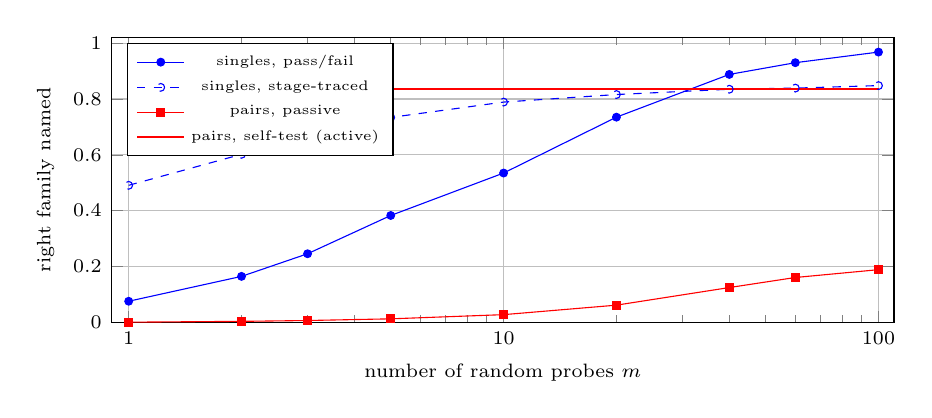
\begin{tikzpicture}
\begin{semilogxaxis}[width=0.95\columnwidth,height=5.2cm,xlabel={number of random probes $m$},ylabel={right family named},xmin=0.9,xmax=110,ymin=0,ymax=1.02,grid=major,tick label style={font=\scriptsize},label style={font=\scriptsize},legend style={font=\tiny,at={(0.02,0.98)},anchor=north west},log ticks with fixed point]
\addplot[blue,mark=*,mark size=1.4pt] coordinates {(1,0.076)(2,0.165)(3,0.246)(5,0.383)(10,0.535)(20,0.735)(40,0.888)(60,0.930)(100,0.968)};
\addlegendentry{singles, pass/fail}
\addplot[blue,dashed,mark=o,mark size=1.4pt] coordinates {(1,0.491)(2,0.602)(3,0.669)(5,0.734)(10,0.789)(20,0.816)(40,0.835)(60,0.839)(100,0.848)};
\addlegendentry{singles, stage-traced}
\addplot[red,mark=square*,mark size=1.4pt] coordinates {(1,0.001)(2,0.004)(3,0.007)(5,0.013)(10,0.028)(20,0.062)(40,0.125)(60,0.161)(100,0.189)};
\addlegendentry{pairs, passive}
\addplot[red,thick,domain=1:100,samples=2] {0.837};
\addlegendentry{pairs, self-test (active)}
\end{semilogxaxis}
\end{tikzpicture}
\caption{Held-out identifiability (seeds 71--73). Passive decoding of single faults improves with more probes and, when probes are few, with stage traces. Pairs stay hard for passive decoding because one fault masks the other; the active self-test names both causes in 83.7\% of effective pairs.}
\label{fig:ladder}
\end{figure}

\subsection{Blind faults: code mutants}\label{sec:res-mutants}
To test the monitor on faults its authors did not design, we mutated the retrieval code itself: relational and arithmetic operators, integer and float constants, negated conditions, swapped variables, deleted statements, operand deletion and configured values off by one, one mutation per mutant, only on lines that a clean query executes. A mutant is harmful if it breaks at least 10\% of 40 working queries. Mutation points were split in half by hash; development used one half, confirmation the other. \textbf{First confirmation (seeds 71--73): insufficient.} The held-out half gave only 6 distinct harmful mutants (16 mutant-seed units), short of the 8 the rule required, because most first-order mutants of this code crash or change nothing. On them, the self-test detected 16 of 16, the stage trace localized the component in 16 of 16 against 9 of 16 for the fault dictionary and 6 of 16 for the most frequent component, and per-query telemetry detected 12 of 16. \textbf{Second confirmation: pass.} On development data we added standard operators (operand deletion, configured value off by one, halved or doubled, swapped conditional branches and \texttt{np.where} arguments) and second-order mutants (two harmless mutants combined; 0 of 150 were harmful on development, so they contribute nothing), and, as a second code base, the second retrieval stack. The rule was unchanged and fixed before the runs: at least 8 distinct scored harmful mutants, detection $\ge0.95$, localization $\ge0.80$ and above both baselines. Table~\ref{tab:mutants} gives the result on the held-out halves (main stack on the untouched pipelines of seeds 74--76, second stack on FiQA): all three conditions hold. Per-query telemetry misses 5 of the 32 harmful runs, mostly mutants that cut or swap the list that is served without changing the scores telemetry reads. On 77 \emph{subtle} mutant runs (1 to 3 of 40 working queries broken), the self-test detects 90\% and telemetry 43\%.

\begin{table}[t]
\caption{Code mutants, held-out halves (second confirmation). Units are mutant runs (a mutant on one pipeline seed); localization is scored on mutants whose code lies in one pipeline stage (17 distinct).}
\label{tab:mutants}
\centering\footnotesize
\begin{tabular}{@{}lcc@{}}
\toprule
 & Main stack & Second stack\\
\midrule
Mutants evaluated (runs) & 644 & 105\\
\quad crash / harmless / subtle & 57 / 503 / 65 & 13 / 67 / 12\\
Harmful runs (distinct mutants) & 19 (8) & 13 (13)\\
Detected by the self-test & 19/19 & 13/13\\
Detected by per-query telemetry & 16/19 & 11/13\\
\midrule
\multicolumn{3}{@{}l}{Localization, both stacks pooled (28 scored runs)}\\
Stage trace & \multicolumn{2}{c}{100\%}\\
Fault-dictionary decoder (main stack, 19 runs) & \multicolumn{2}{c}{47\% (difference $+0.53$ $\ci{+0.18}{+0.89}$)}\\
Most frequent stage & \multicolumn{2}{c}{46\% (difference $+0.54$ $\ci{+0.27}{+0.69}$)}\\
\bottomrule
\end{tabular}
\end{table}

\subsection{Bugs reproduced from public issue reports}\label{sec:res-bugs}
Production incidents are not available to us. The standard substitute in software testing is to reproduce bugs exactly as they were reported in public issue trackers. Before any run we selected nine retrieval-quality bugs that return wrong results silently and whose mechanism can be reproduced on the main stack (Table~\ref{tab:bugs}); seven were never used to design a detector, repair or probe, and two (B8, B9) are the same mechanism as designed faults. Each bug was switched on system-wide and measured on 600 natural ESCI queries that no run had examined. A bug is harmful if it breaks at least 1\% of the natural queries the clean pipeline answers. The self-test ran with 100 random probes; its repair rolls back the localized component to its last verified version and is accepted only if every probe passes.

\begin{table}[t]
\caption{Reproduced bugs on the untouched pipelines of seeds 74, 75, 76. Broken: natural queries (of 337 that the clean pipeline answers) that the bug breaks (identical on every seed). Det.: self-test detection, seeds with an alarm. Stage: localized by the stage trace; all equal the true stage. Repair pass: the finite probe battery. Tel.: seeds on which per-query telemetry alarms. Restored: broken queries that work after the verified repair, summed over seeds.}
\label{tab:bugs}
\centering\footnotesize
\begin{tabular}{@{}llrccr@{}}
\toprule
Bug (report) & Mechanism & Broken & Det. & Tel. & Restored\\
\midrule
B1 dify\#6097 & query prefix dropped & 0 & 0/3 & 0/3 & --\\
B2 rank\_bm25\#50 & query tokenization & 0 & 0/3 & 0/3 & --\\
B3 langchain\#37046 & fusion sums chunks of one source & 7 & 2/3 & 0/3 & 14/21\\
B4 milvus\#53672 & rerank scores misassigned & 13 & 3/3 & 0/3 & 39/39\\
B5 graphiti\#1720 & rerank sorted ascending & 316 & 3/3 & 0/3 & 948/948\\
B6 pygaggle\#67 & rerank order ignored & 46 & 3/3 & 0/3 & 138/138\\
B7 llama\_index cache & previous query's scores reused & 43 & 3/3 & 2/3 & 129/129\\
B8 faiss\#600$^{*}$ & IVF nprobe $=1$ & 42 & 3/3 & 3/3 & 126/126\\
B9 jenkins plugin\#542$^{*}$ & raw-score fusion & 20 & 3/3 & 3/3 & 60/60\\
\bottomrule
\multicolumn{6}{@{}l}{\footnotesize $^{*}$Same mechanism as a designed fault (R15, R22).}
\end{tabular}
\end{table}

Seven bugs are harmful (21 bug-seed units). The pre-registered rule holds on all four conditions: at least 5 distinct harmful bugs (7); self-test detection 20 of 21 (95.2\%); localization to the right stage 21 of 21; every accepted repair verified, 1{,}454 of 1{,}461 broken natural queries restored, and no working query broken by a repair. The miss is B3 on seed 76, which breaks 7 of 337 queries and failed none of that seed's 100 probes, so no repair ran and its 7 queries stayed broken. Per-query telemetry alarms on 8 of 21 units, mostly the two bugs that match designed faults; the per-query loop restores 300 of the 1{,}461 queries and the universal repair 339. The two bugs that break nothing do so for documented reasons: bge-v1.5 is built to work without its query instruction, and ESCI queries are already lower-case. B3 also helps more than it hurts (Hit@5 rises from 56.2\% to 57.8\%), so rolling it back costs 1.7 points net; detection is correct, but whether to roll back is a judgement the self-test cannot make. Under the other six bugs the verified repair raises natural Hit@5 by 1.2 to 48.7 points. Rollback restores exactly the clean pipeline by construction once the stage is right, so the evidence here is detection and localization of bugs nobody designed, and the gap to per-query telemetry (20 against 8 of 21).

\subsection{Real failures and natural traffic}\label{sec:res-real}
\textbf{Natural traffic.} On 1{,}648 ESCI queries no run had examined, the deployed loop gains $+2.0$ to $+2.4$ points of Hit@5 on every seed (seed 50: $+2.43$ $\ci{+1.64}{+3.22}$, 43 fixed, 3 broken). Almost all of it comes from two deterministic rules (near-duplicate and chunk-crowding collapse); classifier dispatch alone adds $+0.42$. Detection decides when the rules fire: gated rules beat the same rule always on by $+0.61$ $\ci{+0.12}{+1.15}$. Repairing natural misspellings hurts ($-4.9$; SymSpell $-11.4$) and is off. The gold document is an empty placeholder for 58.6\% of ESCI queries and 69.1\% of failures, which caps any repair.

\textbf{Real failures labelled by intervention.} A real failure is a natural query whose clean pipeline misses a gold document with content; we ran every repair in the catalogue on it and called it repairable if one restores Hit@5 (no human or model labels). On ESCI, 36 of 215 real failures are repairable (16.7\%). On seeds 71--73 the loop fixes 53 to 58\% of them, against 9\% for a random repair from the catalogue (difference lower bound $+0.28$ or more on each seed) and 69\% for the universal repair. Telemetry detects repairable real failures at AUROC 0.64 to 0.71, reaching the pre-registered 0.70 on one seed of three, and the loop breaks 0.6 to 0.8\% of real successes, above the 0.5\% claim (universal repair 3.8\%). On the second stack only 7\% of real failures are repairable by any repair; the gated loop fixes none of them and breaks none of 1{,}578 real successes, while the universal repair fixes 65 to 81\% and breaks 3.3 to 4.2\%.

\subsection{Unseen faults}\label{sec:res-u1}
Leave-one-fault-out closure of the per-query diagnoser (U1) is 0.36 to 0.41 on every seed, below its 0.50 bar. A ceiling analysis explains most of the gap: with the frozen flagging threshold, only 0.51 to 0.54 of unseen-fault episodes are both flagged and fixable by some repair the per-query system can still choose. A verify-then-escalate policy raised U1 to 0.48 to 0.50 but was not confirmed (mean 0.489; observed harm exceeded 0.5\% on one seed (0.52\%); closure of known faults down to 0.77 to 0.79).

\textbf{The deployed system has two channels.} We therefore measured U1 of the system that runs both the per-query diagnoser and the self-test (pre-registered; no parameter tuned). For each of the 12 system faults among the 25, the self-test runs on the faulted system with a fault dictionary that does not contain that fault; if a probe fails, the candidate repair is applied after it passes the finite battery check; query and content faults keep the per-query outcome. On seed 71, two-channel U1 is \textbf{0.608} against 0.398 for the per-query diagnoser alone ($+0.21$ $\ci{+0.08}{+0.35}$ over faults), above the 0.50 bar; the self-test raised no alarm on the clean system. System faults close 0.96 (per-query 0.52): the self-test detects 11 of the 12 unseen system faults in every episode (K04, which changes only gold vectors, is not seen by the probes) and closes them, by naming a fault of the same repair family for the three encoder faults and by verified rollback to the pinned configuration for the other eight. Query and content faults (13 of 25) stay at 0.28: unseen per-query faults remain open. \PEND{Seeds 72 and 73 were still in the Kaggle GPU queue at the freeze.}

\subsection{Portability of the fault suite}
On the second stack, 19 of 20 ported faults are solved on FiQA (the same 19 on a second seed) and 18 on NQ; K04 is unsolved on both and Q01 on NQ. Most ported detectors sit at AUROC 0.995 or above, so these faults are blunt.

%--------------------------------------------------------------------------------------------------
\section{Limitations}\label{sec:limits}
\textbf{External validity.} No production incident data were available. We address the gap in four ways, none of which replaces field data: 22 of the faults are tied to public field reports by evidence tier; nine bugs are reproduced exactly as reported in public issue trackers (Section~\ref{sec:res-bugs}); code mutants of two retrieval code bases give faults that nobody designed (Section~\ref{sec:res-mutants}); and real failures of natural queries are labelled by which repair fixes them, without human or model judgement (Section~\ref{sec:res-real}). Most real failures are not repairable by any repair in the catalogue (83\% on ESCI, 93\% on the second stack). The main results use one English e-commerce corpus; the second stack (FiQA, NQ) covers 20 of the 32 faults, the per-query risk-control evaluation, the code mutants and the self-test.

\textbf{Natural traffic.} Natural gains are small and come mostly from two rules. On ESCI the gold document is an empty placeholder for 58.6\% of queries, which caps any repair; on the 710 queries whose gold has content the loop gains $+3.24$ points $\ci{+1.97}{+4.51}$ with none broken (seed 50, post hoc).

\textbf{Method limits.} The self-test covers system-wide faults; per-query faults such as typos stay with telemetry, and a fault that breaks almost no probe (R07 on the main stack, K04 on the second) is invisible to it. Its second-stack confirmation uses held-out fault draws on the development corpus, not a new corpus. Unseen-fault closure of the per-query diagnoser misses its bar; the two-channel system meets it on the one seed that finished, mostly through verified rollback of system faults, and unseen query and content faults stay open. Real-failure detection is borderline. Q03 is never identified. The LLM comparison uses free-tier models zero-shot. The capped gate and small-stratum fallback were developed after earlier results; sparse pooled-fallback strata lack a per-stratum guarantee. The self-test's adaptive repair search was not certified on an untouched sample. Five earlier configurations (seeds 42 to 49) preceded the final one; all records are in the repository.

\section{Conclusion}
The per-query conformal gate provides a risk-control target within strata with sufficient calibration data; observed held-out clean losses are low, but pooled-fallback strata do not receive a per-stratum guarantee. Telemetry of one query detects and names injected faults well, but one observation cannot separate two faults of one kind. A known-answer probe battery used actively names both causes of 85\% of same-group pairs on held-out seeds and checks repairs against the finite battery. The adaptive repair search reuses probe outcomes, so its traffic harm is empirical: two of 301 measured repairs exceeded the nominal fixed-candidate 2.95\% value. Active identification uses substantially more probe executions than passive full-battery decoding, and an equal-total-execution comparison was not measured. On automatically generated code mutants selected by the project, the self-test detected every harmful mutant in the evaluated set and its stage trace localized the scored cases.

\section*{Disclosure and Ethics}\label{sec:ethics}
The code, experiments and text were produced with an AI assistant (Claude, Anthropic) under the direction of the authors. [OWNER: replace with the authorship and disclosure wording your venue requires.] No personal data are used; the corpora are public, and no API key is stored in the repository.

\section*{Acknowledgment}
[OWNER: acknowledgments, funding.]

%--------------------------------------------------------------------------------------------------
\begin{thebibliography}{00}
\bibitem{lewis2020rag} P.~Lewis \emph{et al.}, ``Retrieval-augmented generation for knowledge-intensive NLP tasks,'' in \emph{Proc.\ NeurIPS}, 2020.
\bibitem{barnett2024seven} S.~Barnett, S.~Kurniawan, S.~Thudumu, Z.~Brannelly, and M.~Abdelrazek, ``Seven failure points when engineering a retrieval augmented generation system,'' in \emph{Proc.\ CAIN}, 2024, arXiv:2401.05856.
\bibitem{es2023ragas} S.~Es, J.~James, L.~Espinosa-Anke, and S.~Schockaert, ``RAGAS: Automated evaluation of retrieval augmented generation,'' arXiv:2309.15217, 2023.
\bibitem{saadfalcon2024ares} J.~Saad-Falcon, O.~Khattab, C.~Potts, and M.~Zaharia, ``ARES: An automated evaluation framework for retrieval-augmented generation systems,'' in \emph{Proc.\ NAACL}, 2024.
\bibitem{ru2024ragchecker} D.~Ru \emph{et al.}, ``RAGChecker: A fine-grained framework for diagnosing retrieval-augmented generation,'' in \emph{Proc.\ NeurIPS}, 2024, arXiv:2408.08067.
\bibitem{leung2026ragec} K.~K.~Leung \emph{et al.}, ``Classifying and addressing the diversity of errors in retrieval-augmented generation systems,'' in \emph{Proc.\ EACL}, 2026, arXiv:2510.13975.
\bibitem{raglog} [OWNER: authors], ``From logs to faults: Reference-free fault localization for retrieval-augmented generation pipelines (RAGLog),'' arXiv:2611.03725, 2026; code \url{https://github.com/hiraa221/raglog}, commit 7f7d068.
\bibitem{hashemifar2026d2r} S.~Hashemifar, H.~A.~Noughabi, F.~Zarrinkalam, and A.~Dehghantanha, ``Diagnosing and repairing factual errors in RAG under budget constraints,'' arXiv:2606.29377, 2026.
\bibitem{pothuru2026agenticfp} L.~Pothuru, ``When failures propagate: Causal failure attribution in agentic retrieval-augmented generation,'' in \emph{REALM Workshop, EMNLP}, 2026, arXiv:2608.20627.
\bibitem{yan2024crag} S.-Q.~Yan, J.-C.~Gu, Y.~Zhu, and Z.-H.~Ling, ``Corrective retrieval augmented generation,'' arXiv:2401.15884, 2024.
\bibitem{kim2026metamorphic} [OWNER: verify authors] ``When knowledge changes: Metamorphic testing of RAG systems with mutations,'' arXiv:2607.26843, 2026.
\bibitem{angelopoulos2024crc} A.~N.~Angelopoulos, S.~Bates, A.~Fisch, L.~Lei, and T.~Schuster, ``Conformal risk control,'' in \emph{Proc.\ ICLR}, 2024.
\bibitem{vovk2013mondrian} V.~Vovk, ``Conditional validity of inductive conformal predictors,'' \emph{Machine Learning}, vol.~92, 2013.
\bibitem{kang2024crag} M.~Kang, N.~M.~G\"urel, N.~Yu, D.~Song, and B.~Li, ``C-RAG: Certified generation risks for retrieval-augmented language models,'' in \emph{Proc.\ ICML}, 2024.
\bibitem{opoku2026toolchain} J.~Opoku and D.~Banahene, ``ToolChain-CRC: Conformal risk control for agentic AI under retrieval and tool-use drift,'' arXiv:2606.18467, 2026.
\bibitem{reiter1987theory} R.~Reiter, ``A theory of diagnosis from first principles,'' \emph{Artificial Intelligence}, vol.~32, no.~1, pp.~57--95, 1987.
\bibitem{dekleer1987diagnosing} J.~de~Kleer and B.~C.~Williams, ``Diagnosing multiple faults,'' \emph{Artificial Intelligence}, vol.~32, no.~1, pp.~97--130, 1987.
\bibitem{sampath1995diagnosability} M.~Sampath, R.~Sengupta, S.~Lafortune, K.~Sinnamohideen, and D.~Teneketzis, ``Diagnosability of discrete-event systems,'' \emph{IEEE Trans.\ Autom.\ Control}, vol.~40, no.~9, pp.~1555--1575, 1995.
\bibitem{dorfman1943} R.~Dorfman, ``The detection of defective members of large populations,'' \emph{Ann.\ Math.\ Statist.}, vol.~14, no.~4, pp.~436--440, 1943.
\bibitem{du2000group} D.-Z.~Du and F.~K.~Hwang, \emph{Combinatorial Group Testing and Its Applications}, 2nd~ed. World Scientific, 2000.
\bibitem{shwe1991qmr} M.~A.~Shwe \emph{et al.}, ``Probabilistic diagnosis using a reformulation of the INTERNIST-1/QMR knowledge base,'' \emph{Methods Inf.\ Med.}, vol.~30, 1991.
\bibitem{bushnell2000essentials} M.~L.~Bushnell and V.~D.~Agrawal, \emph{Essentials of Electronic Testing for Digital, Memory and Mixed-Signal VLSI Circuits}. Kluwer, 2000.
\bibitem{just2014mutants} R.~Just, D.~Jalali, L.~Inozemtseva, M.~D.~Ernst, R.~Holmes, and G.~Fraser, ``Are mutants a valid substitute for real faults in software testing?'' in \emph{Proc.\ FSE}, 2014, pp.~654--665.
\bibitem{jia2011survey} Y.~Jia and M.~Harman, ``An analysis and survey of the development of mutation testing,'' \emph{IEEE Trans.\ Softw.\ Eng.}, vol.~37, no.~5, pp.~649--678, 2011.
\bibitem{jia2009hom} Y.~Jia and M.~Harman, ``Higher order mutation testing,'' \emph{Inf.\ Softw.\ Technol.}, vol.~51, no.~10, pp.~1379--1393, 2009.
\bibitem{pearl2009causality} J.~Pearl, \emph{Causality}, 2nd~ed. Cambridge Univ.\ Press, 2009.
\bibitem{clopper1934} C.~J.~Clopper and E.~S.~Pearson, ``The use of confidence or fiducial limits illustrated in the case of the binomial,'' \emph{Biometrika}, vol.~26, no.~4, pp.~404--413, 1934.
\bibitem{shtok2012qpp} A.~Shtok, O.~Kurland, D.~Carmel, F.~Raiber, and G.~Markovits, ``Predicting query performance by query-drift estimation,'' \emph{ACM Trans.\ Inf.\ Syst.}, vol.~30, no.~2, 2012.
\bibitem{zhou2007wig} Y.~Zhou and W.~B.~Croft, ``Query performance prediction in web search environments,'' in \emph{Proc.\ SIGIR}, 2007.
\bibitem{xiao2023bge} S.~Xiao, Z.~Liu, P.~Zhang, and N.~Muennighoff, ``C-Pack: Packaged resources to advance general Chinese embedding,'' arXiv:2309.07597, 2023.
\bibitem{robertson2009bm25} S.~Robertson and H.~Zaragoza, ``The probabilistic relevance framework: BM25 and beyond,'' \emph{Found.\ Trends Inf.\ Retr.}, vol.~3, no.~4, 2009.
\bibitem{cormack2009rrf} G.~V.~Cormack, C.~L.~A.~Clarke, and S.~Buettcher, ``Reciprocal rank fusion outperforms Condorcet and individual rank learning methods,'' in \emph{Proc.\ SIGIR}, 2009.
\bibitem{reddy2022esci} C.~K.~Reddy \emph{et al.}, ``Shopping queries dataset: A large-scale ESCI benchmark for improving product search,'' arXiv:2206.06588, 2022.
\bibitem{hagen2017qspell} M.~Hagen, M.~Potthast, M.~Gohsen, A.~Rathgeber, and B.~Stein, ``A large-scale query spelling correction corpus,'' in \emph{Proc.\ SIGIR}, 2017.
\bibitem{thakur2021beir} N.~Thakur, N.~Reimers, A.~R\"uckl\'e, A.~Srivastava, and I.~Gurevych, ``BEIR: A heterogeneous benchmark for zero-shot evaluation of information retrieval models,'' in \emph{NeurIPS Datasets and Benchmarks}, 2021.
\bibitem{pedregosa2011sklearn} F.~Pedregosa \emph{et al.}, ``Scikit-learn: Machine learning in Python,'' \emph{J.\ Mach.\ Learn.\ Res.}, vol.~12, 2011.
\bibitem{wilson1927} E.~B.~Wilson, ``Probable inference, the law of succession, and statistical inference,'' \emph{J.\ Am.\ Stat.\ Assoc.}, vol.~22, no.~158, 1927.
\end{thebibliography}

\end{document}
